\documentclass{article}
\usepackage[utf8]{inputenc}
\usepackage{graphicx}
\begin{document}
\section{ Processamento de linguagens }

\subsection{ Título nível 2 }

\subsubsection{ Título nível 3 }


\section{ Tabelas }

\begin{table}[h]
\begin{tabular}{|l|l|l|l|}
\hline

Coluna 1  &  Coluna 2  &  Coluna 3  &  Coluna 4 \\ \hline
2  &  3  &  4  &  5 \\ \hline
4  &  5  &  6  &  7 \\ \hline


\end{tabular}
\end{table}


Exemplo de texto em \textbf{negrito}. 

Exemplo de texto em \textit{italico}.

\section{ \textit{ Listas } }

\subsection{ Lista padrão }
Lista:

\begin{itemize}
 
	
	\item  elemento 1
	
	\item  elemento 2
	
	\item  elemento 3
	
	\item  \textbf{ elemento a negrito na lista }

\end{itemize}

	- elemento fora do contexto de lista

\subsection{ Lista numerada }

Lista:

\begin{enumerate}
 
	
	\item  elemento 1

	
	\item  elemento 2

	
	\item  elemento 3

	
	\item  
\textbf{ elemento a negrito na lista }
\end{enumerate}

\section{ Imagens }
	
\begin{figure}[h]
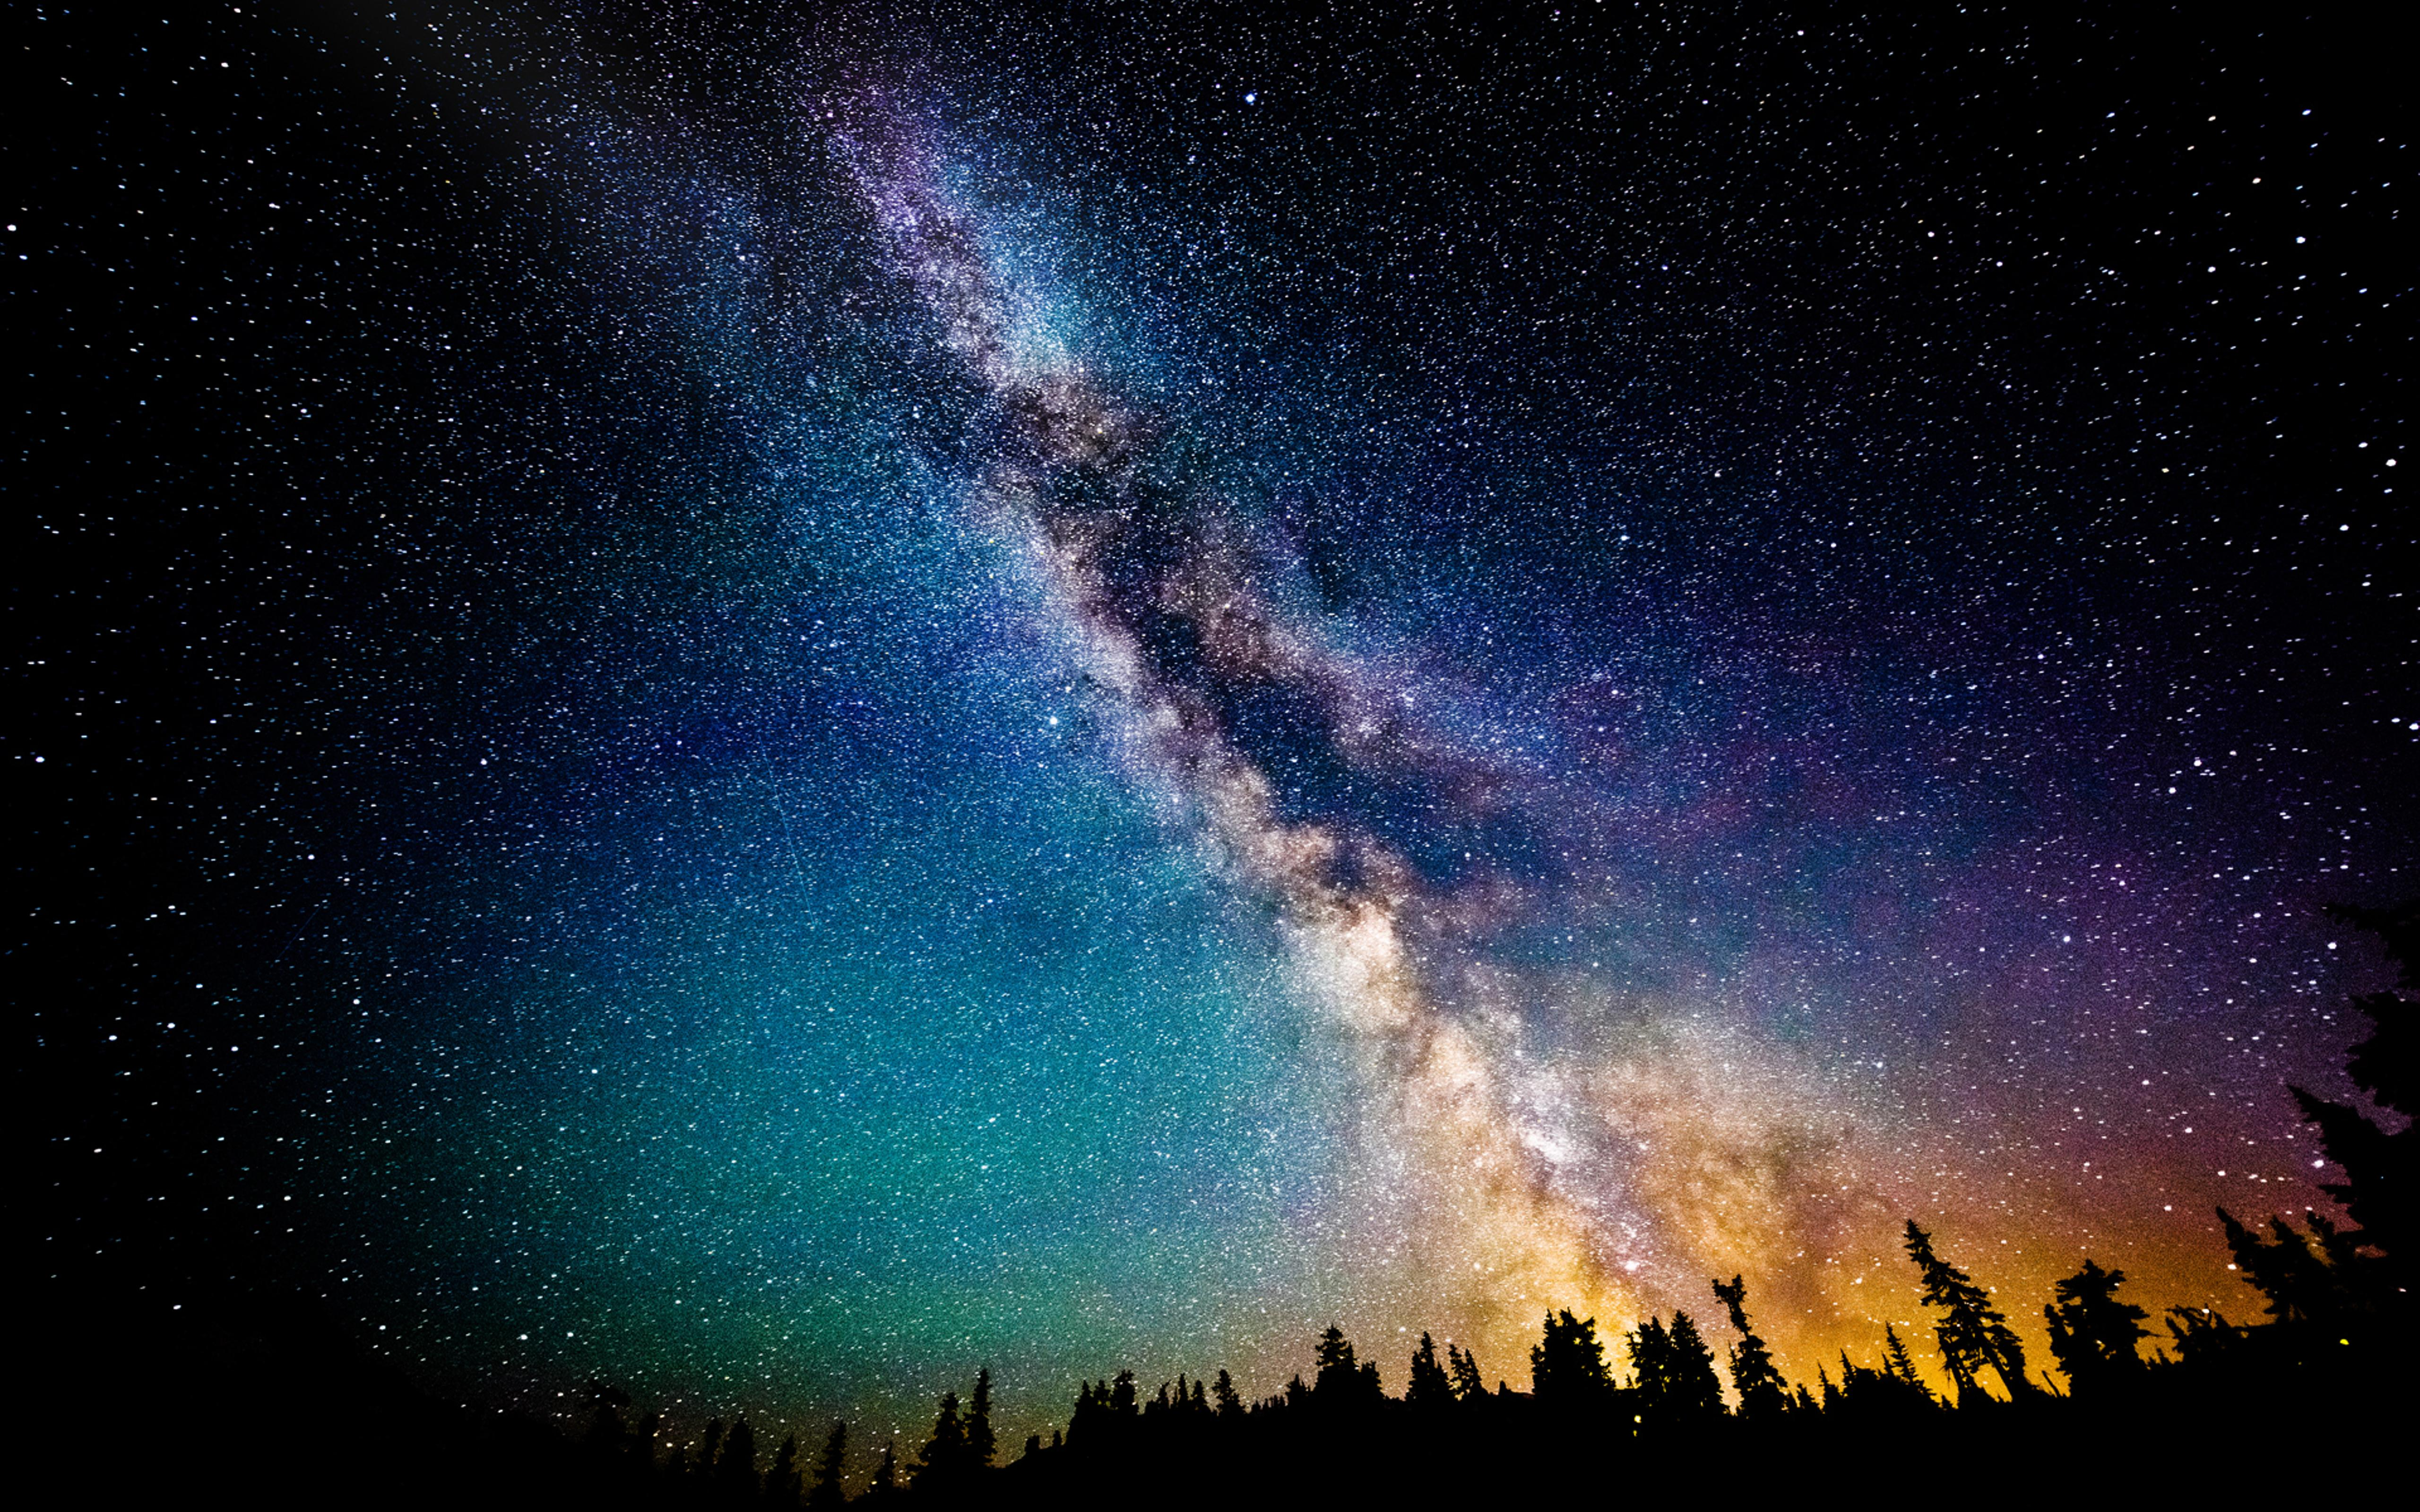
\includegraphics[width=400px]{ Image1.jpg }

\end{figure}


\begin{figure}[h]

\includegraphics[width=400px]{ Image2.jpg }
\caption{ Legenda da imagem 2 } 
\end{figure}


\begin{figure}[h]

\includegraphics[width=400px]{ Image3.jpg }
\caption{ Legenda da imagem 3 com \textit{ italico } e \textbf{ negrito } e caracteres especiais \% \$ } 
\end{figure}




\end{document}
